\documentclass[conference]{IEEEtran}
\usepackage{fancyhdr}\usepackage[utf8]{inputenc}
\usepackage{graphicx}
\usepackage{multirow}

\usepackage{lastpage}

%\usepackage{draftwatermark}


%\SetWatermarkText{UoA}
%\SetWatermarkScale{3}

\pagestyle{fancy}
\fancyhf{}
\rfoot{Page \thepage \hspace{1pt} of \pageref{LastPage}} 

\title{Is it possible to extend IPv6?}
\date{December 2022}

\author{\IEEEauthorblockN{Ana Custura}
\IEEEauthorblockA{
\textit{University of Aberdeen}\\
}
\and
\IEEEauthorblockN{Raffaello Secchi}
\textit{University of Aberdeen}\\
\and
\IEEEauthorblockN{Gorry Fairhurst}
\textit{University of Aberdeen}\\
}
\begin{document}

\maketitle

\begin{abstract}
The IPv6 Hop-by-Hop Options and Destination Options Extension Headers have historically faced challenges in deployment due to the lack of support in hardware-based forwarding and concerns around potential denial-of-service attacks. However, there has been a renewed interest within the standards community both in simplifying their processing, and in using them for new applications. 
Through a wide-scale measurement campaign, we show that many Autonomous Systems (ASes) in access networks and core of the Internet permit the traversal of EHs carrying options, and that path traversal is highly variable depending on the type of network, size of option and transport protocol used, but not on the type of option sent. We also show that packets with Extension Headers can impact load balancing network functions, and present evidence of equipment misconfiguration. Finally we outline the remaining deployment challenges for the EHs and provide recommendations for utilizing them.

\end{abstract}

\begin{IEEEkeywords}
IPv6 protocol, Extension Headers, Protocol Evolution
\end{IEEEkeywords}

\section{Introduction}
\label{sec:introduction}

IPv6 Extension Headers (EHs)~\cite{RFC8200} are optional headers that can be 
added to the base IPv6 header to provide extra functionality and features in
IPv6 networks. They were included in the original IPv6 specification
to make the protocol flexible and extensible.
%The use of extension headers allows for a flexible and extensible design of IPv6 that can support a variety of new networking features and technologies.
% commented out as it does not say much
Despite the potential benefits of IPv6 EHs, studies have shown that their use
has not been widespread~\cite{rfc9098}. A reason often cited for this is that many
network devices, such as firewalls and routers, do not properly handle packets
containing extension headers, which can cause interoperability issues.
Additionally, some network administrators may firewall extension
headers due to security concerns, as they have historically been used to bypass
security mechanisms or launch Denial of Service (DoS) attacks~\cite{naagas2021deh}.

A plausible process that has resulted in the limited usage of IPv6 EHs
has recently been described in a draft Internet standard~\cite{ietf-v6ops-hbh-03}. Authors claims  that early routers
predominantly processed EHs in software, as ASIC implementations for processing
them were scarce. Consequently, the processing of EHs occurred
primarily in the control plane of routers, requiring longer processing
(slow-path) and computing times, and leading to a decrease in throughput.  To
overcome this challenge, network operators began to disable EH processing in their
networks, or even dropping packets with EHs altogether.  In turn, this
discouraged their development within the standards community and further integration
with other network technologies.

Taking this viewpoint into account, this paper demonstrates the wider
accessibility of EH processing in modern routers. By utilising results from two
extensive measurement campaigns, we illustrate that IPv6 routers are now more
capable in handling EHs.  However, our findings also reveal
that there are still prevalent pathologies in certain Internet areas that challenge the further adoption of IPv6 EHs.

This paper begins by discussing various separate measurements reporting
potentially contrasting results on IPv6 path traversal rates~\cite{RFC7872}
\cite{apnic} \cite{nalini-iepg114} \cite{james}.  Discrepancies in individual
studies are here attributed to either too narrow datasets or a focus
on overly specific scenarios.  With the use of broader datasets and the
consideration of various factors, including packet lengths, header lengths,
transport type, and packet composition, we paint a more diverse and nuanced
picture of Internet paths than was previously thought.

Specifically, our research demonstrates that if the EHs are limited in size,
packets carrying Destination Options can traverse as many as
95\% of a diverse set of Internet paths. However, packets carrying a Hop-by-Hop Options EH only traverse a very narrow set of paths. On the other hand, when we
characterise whether these packets traverse Autonomous Systems (AS), if we exclude operator policies in access and transit networks, we find many ASes allow transparent forwarding of EHs.

This paper also presents novel insights into how the inclusion of EHs in packets
impacts the forwarding process from source to destination. Our research findings
demonstrate that the inclusion of EHs in packets on paths with some form of network layer load-balancing often results in a narrower set of forwarding paths. Although one could interpret this as an
alternative approach to extracting entropy from EHs, it is more likely a
pathological outcome of load balancing network devices not properly equipped
to handle packets carrying EHs.

We claim that eliminating these pathologies would open up opportunities for
developers and network operators to take advantage of a range of recently-standardised or in-progress innovative ideas based on EHs, such as sending larger packets~\cite{rfc9268} or monitoring network
performance~\cite{rfc8250}~\cite{ietf-ippm-ioam-ipv6-options-10}.

The rest of the paper is organised as follows:  Section~\ref{sec:background} presents
the required background on IPv6 EHs and the historical challenges related to
their deployment.  The previous literature on IPv6
EH measurements of is surveyed in Section~\ref{sec:motivation}.
Sections~\ref{sec:methodology}-\ref{sec:pathspider-results} present the
methodology and results of this study, organised by type of network path.  The
implications of our results are discussed in Section~\ref{sec:discussion}.
Finally the conclusion summarises our findings.

\section{IPv6 Preliminaries}
\label{sec:background}

\label{sec:ipv6-option-deployment}

\begin{figure}
\centering
  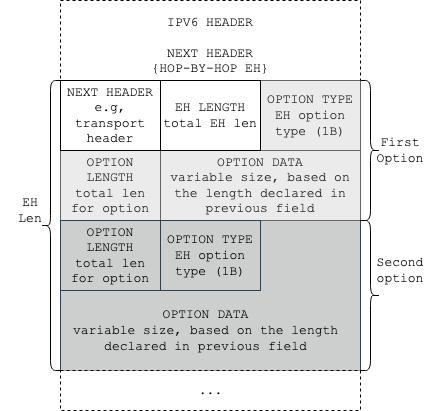
\includegraphics[width=0.5\textwidth]{ehformat.png}
  \caption{IPv6 packet with base header and two EHs}
  \label{fig:eh-format}
\end{figure}


IPv6~\cite{rfc2460} introduces a flexible header structure consisting of a
fixed-length base header followed by optional Extension Headers (EHs). 
The type of the very first EH in the chain is specified in the Next Header field of the IPv6 base header, and each consecutive EH contains a Next Header field to specify the type of the next EH in the chain or the presence of an IPv6 payload. Each EH also contains a Length field specifying its total length.
Types of EHs include Hop-by-Hop Options (HbH Opts), Routing, Fragment, and
Destination Options (Dest Opts).  RFC 8200~\cite{RFC8200} allows any sequence
of EHs in a single packet as long as they can fit the first fragment in case of
fragmentation.

Dest Opts are meant to be consumed at the destination, and propagated
transparently by intermediate devices on a given path. All the other EHs, instead, carry
information relevant to packet forwarding and should be processed along the
path. To simplify processing by routers, RFC 8200 also requires inserting HbH
Opts immediately after the base header.

Figure~\ref{fig:eh-format} shows the structure of an IPv6 packet including a base
header followed by a HbH Options EH containing two Options.  Each Option uses the same Type-Length-Value (TLV) encoding~\cite{RFC8200} with 1~byte each allocated for the Type and Length fields and a variable-size Value field to carry option data. Altough EHs are variable size headers, their length is always a multiple of 8 bytes to preserve alignment.

Encoding the Type and Length fields using fixed-length allows an IPv6
router to skip options it does not understand. In
addition, when an option is unknown, the two most significant bits of the Type
specify the action the device should take to address the unrecognised header.
In particular, if the two most significant bits are 00, the device should
ignore the option and continue processing the header. If these bits are 01, the
processing should stop and the packet discared. If the bits are 10,
the packet should be discarded and an ICMP notification should be returned to
the sender. Finally, if the bits are 11, the same actions as 10 should occur
but the notification should be sent only if the destination address was not
multicast. 

Table~\ref{tbl:options} presents the options currently standardised.  We note
that the most common choice options is to set the two most significant bits
(MSBs) to 00.  The third most significant bit instead specifies, if set, 
that the option data field can be modified en route.


Because they can be modified individually by network devices on a path, packets
with HbH Opts have measurement applications within a network domain. They can
be used in place of traditional mechanisms for measurement that rely on ICMP:
Option 0x30 has been defined as alternative to PMTUD~\cite{rfc9268}, option
0x12 has been specified to measure packet loss, latency, and jitter on live
traffic measurements~\cite{rfc9343} and recently-proposed option 0x31 records
operational and telemetry information that can be updated by devices on the
path between two endpoints. Dest Opts can provide some similar functionality
between endpoints - option 0x0F~\cite{rfc8250} can be used to measure
performance and diagnostic metrics like round-trip delay.  Other applications
for packets with HbH Opts include improving the reliability of packet
forwarding in lossy networks.

Originally all devices on a path were required to examine and process the HbH
Opts header~\cite{rfc2460}. This requirement was updated by~\cite{RFC8200} to
only apply to devices that have been explicitly configured to process it.


% The total EH length is 8-byte aligned and specified in the
% EH Length field, while each individual option declares its own length in the
% Option Length field. 

\begin{table}[b]
\center
\caption{Standardised Dest and HbH Option.}
\begin{tabular}{p{0.03\textwidth}|p{0.055\textwidth}|l|p{0.18\textwidth}}
Hex  & MSBs & Type      & Description                                              \\
\hline
\hline
0x00 & 000  & HbH, Dest & Pad1 (padding)                                           \\
0x01 & 000  & HbH, Dest & PadN (padding)                                           \\
0xC2 & 110  & HbH       & Enable jumbo payloads                                    \\
0x23 & 001  & HbH       & Low-Power and Lossy Networks routing                     \\
0x04 & 000  & Dest      & Mechanism for IPv6 encapsulation                 \\
0x05 & 000  & HbH       & Mechanism for requesting router processing, Router Alert              \\
0xC9 & 110  & Dest      & Mobility Support in IPv6                                 \\
0x8C & 100  & Dest      & Method for identifying subscribers in broadband networks \\
0x6D & 011  & HbH       & Multicast Protocol for Low-Power and  Lossy Networks     \\
0x0F & 000  & Dest      & Delay measurement                                        \\
0x30 & 001  & HbH       & Path MTU measurement                                     \\
0x11 & 000  & HbH, Dest & \multirow{2}{*}{On-path operational info}                \\
0x31 & 001  & HbH, Dest &                                                          \\
0x12 & 000  & HbH, Dest & On-path telemetry                                       
\end{tabular}
  \label{tbl:options}
\end{table}


\subsection{Previous Studies of IPv6 EHs}

\label{sec:motivation}

The debate on the whether or not IPv6 packets with EHs traverse the Internet is not new to the Internet community.

In 2015, an Informational IETF document presenting traceroute active
measurements to destinations within the Alexa top 1M domains~\cite{RFC7872}
revealed that packets with EHs experience significantly higher drops over the
Internet than packets without EHs. Since then, other
studies~\cite{james}~\cite{nalini-iepg114}~\cite{apnic} have appeared within the standards community in
support of this claim.  However,
the level and nature of the reported disruption varied significantly in these
reports.  This called for more analysis into the causes of the limited EH
support and the definition of new investigation methods~\cite{james}~\cite{elkins-v6ops-eh-deepdive-fw-01}.  

A recent IETF draft~\cite{elkins-v6ops-eh-deepdive-fw-01} proposes a new
methodology for isolating the reasons behind EH packet drops and pinpoint the
responsible devices. This draft focuses particularly on cases where the tested
server is behind a CDN (Content Delivery Network).  While no measurement are included in this document, the authors reported separately on a successful FTP experiment with enabled Dest Opts between 6 vantage points~\cite{nalini-iepg114}.

Another recent IETF draft, Just Another Measurement of Extension header
Survivability (JAMES)~\cite{james}, presents results on EH path traversal using
traceroute measurements over a mesh network with 21 vantage points located in globally distributed Autonomous Systems (ASes). This study tests all standardised EHs
(including Routing, Fragment, etc.) in a setting where both ends of the
communication path are under the control of the researcher.  The study found
that only 8-9\% of path support an 8B HbH Option, and a 97\% traversal for 8B
Dest Opts, with traversal rates decreasing as the size of the EH
increases~\cite{james-imc}.  We note 6 of the 21 vantage points were
hosted by Digital Ocean\texttrademark, a Cloud provider that does not support
HbH Options through their networks.

An innovative measurement methodology to analyse end-to-end path traversal
rates of Fragmentation, HbH and Dest Opts was introduced by engineers in
APNIC~\cite{apnic}.  This technique consists in initiating TCP connections from
clients using a crowd-sourced approach and perform end-to-end
measurements by replying with packets including an EH. If the client then replies to the EH packet, the test is considered successful.  APNIC reports a volume of 4M measurements/day from clients across most of the IPv6 internet. Their findings show clients reply 50\% of the time for Dest Opts and close to zero for HbH Opts. We note that this test does not simply measure traversal over Internet paths, but also whether or not end-user devices reply to a packet with Options. 
%We also note that all measurements were performed from servers in a
%single Cloud provider (Linode).

% The different results outlined above present conflicting views, representative
% of the complex nature of Internet paths. We argue the differences are explained
% by examining the types of networks measured and the choice of vantage points
% and destinations. To fully explore the various aspects of EH traversal, our
% work takes a large-scale measurement approach, testing a wide range of access,
% core and server edge networks, and focuses on the HbH and Dest Opts EH types.
% In Section~\ref{sec:discussion}, our results from measurements in access
% networks are compared and discussed alongside their closest counterpart - the
% measurements presented in JAMES~\cite{james}. As we also test edge paths to
% target servers based on top 1M domains lists, we refresh the data presented
% in~\cite{RFC7872} for a longitudinal view.

A large passive measurement campaign carried over the Czech Republic national
research and education network analysed IPv6 traffic over a period of a month in
2016~\cite{passive-threats}. It was found that 0.1\% of IPv6 flows
contained an EH, out of which 40.9\% were HbH Opts packets carrying ICMPv6
payloads, primarily multicast (although not specified by the original authors,
we note this to be Multicast for Low-Power and Lossy Networks~\cite{RFC7731}).
The study notes that dropping ICMPv6 traffic containing EHs could result in
loss of essential network control information. 

% With the exception of~\cite{james-imc}, there are no other peer-reviewed active
% measurement studies. 

Our large-scale measurement study complement previous analysis in that not only
looks at the end-to-end support in servers, but also provides comparative path
analysis and longitudinal changes for HbH and Dest Opts EHs.

\subsection{Challenges and Operational Considerations}

The parsing of IPv6 packets with EHs depends on a device implementation and
architecture. As the Internet emerged and became widespread, routers started having a split architecture with a control and forwarding plane~\cite{RFC3654}, corresponding to router-critical operations running in software and hardware processing respectively.
%In this architecture, incoming packets can be processed on the ``fast path" in the forwarding plane on an Application Specific Integrated Circuits (ASIC) or sent for processing over an internal link on the ``slow path", or the control plane of a router. 

As IPv6 emerged, many network device architectures processed packets containing IPv6 EHs in the ``slow path"~\cite{ietf-v6ops-hbh-03}.  This resulted in opening these routers up to DoS attacks~\cite{naagas2021deh}, as clients sending a large amount of IPv6 traffic with EHs could affect a router's control plane functions where no rate-limiting of such packets was available. This steered
network operators to configure their devices to discard packets containing EHs,
in particular the HbH Opts EH~\cite{ietf-v6ops-hbh-03}. This filtering remains a challenge to EHs deployment.

Another existing challenge relates to implementations within network devices that need to identify the upper-layer protocol header of a packet. This
requires parsing the entire IPv6 header chain from the base header to
the last EH. These devices are common in the network domain edge,
and include routers implementing Access Control Lists (ACLs) or Equal Cost
Multipath Routing (ECMP), and equipment that performs functions such as
application load balancing, Multifield (MF) classification, deep packet
inspection (DPI) or Denial of Service (DoS) attack mitigation. These devices may also discard packets with EHs due to buggy implementations or security considerations.


A different set of considerations applies to network devices that operate in the Internet core, which typically do not require any flow information.
RFC 9288~\cite{rfc9288} produced a set of recommendations for transit routers. While the document recommends permitting packets with the Dest Opts EH, for HbH Opts, the recommendation is to allow the forwarding of packets where they can be forwarded on the fast path, or where on the slow path as long as rate-limiting is available. Where no mitigation options are present, the recommendation is to discard packets containing these headers. 

%In the early Internet, packet routers were implemented entirely
%in software, and as the Internet grew packet processing was moved from software
%to Application Specific Integrated Circuits (ASICs), while the control
%functions remained~\cite{router-architecture}. Routers started having a split
%architecture with a control and forwarding plane~\cite{RFC3654}, corresponding
%to router-critical operations running in software and hardware processing
%respectively. 
%In this architecture, incoming packets can be processed on the
%``fast path" in the forwarding plane on an ASIC or sent for processing over an
%internal link on the ``slow path", or the control plane of a router. 

%As IPv6 emerged, ASIC support for it was limited, and IPv6 deployment itself was in its infancy - and many network device architectures processed packets containing IPv6 EHs in software~\cite{ietf-v6ops-hbh-03}.  This resulted in opening these routers up to DoS attacks~\cite{naagas2021deh}, because clients sending a large amount of IPv6 traffic with EHs could affect a router's control plane functions where no rate-limiting of such packets was available. This steered
%network operators to configure their devices to discard packets containing EHs,
%in particular the HbH Opts EH~\cite{ietf-v6ops-hbh-03}.

%https://ieeexplore.ieee.org/stamp/stamp.jsp?tp=&arnumber=7949061

%\subsection{Hop-by-Hop and Destination Option EHs}

%An IPv6 packet can contain zero or more EHs, each identified by its own number
%in the Next Header field in the preceding header. The HbH Opts header is
%indicated by the value 0, while the assigned protocol number for the Dest Opts
%header is 60. Both HbH and Dest Opts can be included in the same IPv6 packet in
%different EHs. An EH can contain multiple Options - Figure~\ref{fig:eh-format}
%presents one EH with 2 Options.


% Although intended to be
% processed differently, HbH and Dest Opts EHs carry a variable number of Options
% that share the same Type-Length-Value (TLV) encoding~\cite{RFC8200}. Option
% Type and Length are each encoded within one Byte, followed by a variable-size
% Option Value field that carries the option data. Figure~\ref{fig:eh-format}
% shows this format. The total EH length is 8-byte aligned and specified in the
% EH Length field, while each individual option declares its own length in the
% Option Length field. Standardized option types are presented in
% Table~\ref{tbl:options}.

% Please add the following required packages to your document preamble:



%\subsection{Operational considerations}

%\textbf{POSSIBLY MOVE THIS SECTION BELOW}



\section{Methodology} 
\label{sec:methodology}

This paper employs a combination of tools and experiments to delve into various aspects of HbH and Dest Opts traversal. Table~\ref{tbl:datasets} presents the purpose and name of each resulting dataset, alongside the time periods each measurement was ran and the transport protocols that it used.

\begin{table}
\begin{tabular}{p{0.17\textwidth}|p{0.075\textwidth}|p{0.03\textwidth}|p{0.065\textwidth}|p{0.03\textwidth}}
Purpose                                                                          & Tool Used        & Name & Date               & Trans. \\
\hline
Explore traversal of 8B Opts in access networks                                  & Traceroute       & R1           & Oct 2022- Jan 2023 & UDP TCP          \\
\hline
Explore traversal and EH size in access networks                                & Traceroute       & R2           & Oct 2022           & UDP TCP          \\
\hline
Explore if packets with Opts take the same Internet path as vanilla packets & Paris Traceroute & R3           & Jan 2023           & UDP               \\
\hline
Explore traversal of Opts to the server edge                              & PATHSpider       & P1           & Jul 2020- Jan 2023 & UDP TCP          \\
\hline
Explore if variations in Opt type, length or content affects EH traversal   & PATHSpider       & P2           & Jul 2022- Dec 2022     & UDP              
\end{tabular}
  \caption{Experiments and Datasets}
  \label{tbl:datasets}
\end{table}

Experiment setups are discussed in the next subsections.

    \subsection{RIPE Atlas - access network paths}
    \label{sec:ripe-methodology}

Datasets R1-R3 in Table~\ref{tbl:datasets} were collected using RIPE Atlas~\cite{bajpai2015lessons}.
The RIPE Atlas measurement platform was chosen for this study due to its large number of IPv6 vantage points and its ability to perform Paris Traceroute measurements with the PadN Option defined for the Dest and HbH EHs. This option was defined in the original IPv6 standard and its purpose is to pad an EH to ensure 8B alignment, and so is expected to be recognised by most IPv6 implementations.
RIPE Atlas supports setting the size for both types of EHs when performing measurements. At the time of writing, the platform provides 5464 IPv6 vantage points (probes) across 644 unique Autonomous System Numbers, spanning a range of commercial ISPs and R\&E access networks. The number of probes available fluctuates as volunteer-run probes in edge networks can become disconnected over time.

We collected traceroutes from all available vantage points on the platform, using both Dest and HbH Opts EHs of 8 Bytes in size, and in each case using UDP and TCP as the underlying transport, to 7 different globally distributed target servers (dataset R1), without varying the source port and flow label. Baseline UDP and TCP measurements using vanilla IPv6 packets (without an EH) were also collected for each target.
A separate experiment keeps the destination country fixed, but varies the transport and size of EH between 8 and 64B (dataset R2).

Finally, we use RIPE Atlas to perform Paris Traceroute~\cite{augustin2006avoiding} measurements, aiming to detect whether using an EH impacts the path taken between a vantage point and destination. We only select vantage points where traversal is successful over UDP for both types of tested EH to a specific target, ensuring a total of 866 complete paths are measured.
We measure these paths using vanilla IPv6 packets, and packets carrying 8 Bytes Dest and HbH Opts EHs. Each measurement is repeated 16 times, with each repetition varying the source port and flow label of the traceroute packets. Each repetition is assigned a Paris ID to identify it. Finally, we repeat each set of 16 Paris measurements 5 times (dataset R3).


    \subsection{PATHSpider - server edge paths}
    \label{sec:pathspider-methodology}

We use PATHSpider~\cite{learmonth2016pathspider}, a tool for path transparency testing, to survey IPv6-enabled Domain Name System (DNS) servers over multiple years (2019-2023) from the same vantage point located at the University of Aberdeen. At the time this experiment was started, the targets were the IPv6 authoritative Name Servers (NS) for the then-current Alexa Top 1M domains list, and PATHSpider did not have the capability to perform the test over TCP. The longitudinal measurement therefore only presents UDP results, and reuses the same set of domains to avoid changes introduced by continuously tracking a Top 1M Domains list. The domains are resolved again prior to each measurement, and any duplicate or unreachable addresses are removed, resulting in between 19,000 and 22,000 unique IPv6 addresses per measurement.

We extend PATHSpider to support measurements over TCP and repeat this test in 2023 using both transports from 5 globally distributed vantage points to both DNS and webservers extracted from the latest version of Cisco Umbrella Top 1M Domains (19054 and 232350 unique IP addresses respectively). When TCP is measured, the EH is inserted on the first packet (the TCP SYN) and all subsequent packets in the connection.
The test also records whether any ICMP messages are received. This allows us to understand if servers on the path dropping EH packets are configured to send ICMP Unreachable messages.

In the latter test, we also vary the Option Type and declared Option Length fields (dataset P2). This allows us to observe whether different types of options, or incorrectly declared lengths affect EH traversal. For these tests, we also record any ICMP messages received at the sender for a source-destination pair, with the goal of understanding how often ICMP Type 3 (Destination Unreachable) or ICMP Type 4 (Parameter Problem) messages are sent by routers that drop packets carrying an EH. To measure the latter, we ensure one tested Option Types has the highest order bits set to 11, presented in Table~\ref{tbl:options}.

For the server-side measurements described above, the targets selected are DNS servers, due to their ability to be surveyed using both UDP and TCP, although we also present traversal results for the webservers underpinning the Cisco Umbrella top 1M domains.

The following section separately presents the RIPE Atlas access network and PATHSpider server edge results.

\section{RIPE Atlas results} 
\label{sec:ripe-results}

This section presents results obtained using the RIPE Atlas measurement platform, using up to 5000 vantage points towards 8 destinations, of which half are under the control of the researcher. The section primarily reports on the the percentage of paths where test packets were observed to reach the destination AS (the traversal rate). Packets not reaching the destination AS are inferred to be dropped. 

\subsection{Traversal to destination AS}

%Prior to each test case, a baseline measurement using vanilla packets was carried out and unreachable probes were subsequently removed from the result set. 
Figure~\ref{fig:countrybox} shows aggregated traversal results measuring targets in 7 different countries: US, UK, Australia, Poland, Zambia, Kazakhstan and Singapore, from an average of 4750 vantage points. This figure demonstrates the type of EH, transport protocol and choice of destination can affect traversal.

A PadN Dest Opts EH of 8 Bytes (B) in size sees a much higher overall traversal rate compared to the same HbH Opts EH. Similarly, the UDP transport protocol sees a higher traversal rate compared to TCP. Packets with Dest Opts traverse a median of 83\% of the paths tested over UDP and 57\% over TCP, whilst packets with HbH Opts only traverse a median of 12 and 9\% of paths over UDP and TCP respectively.
The spread of values for each EH-transport combination seen in Figure~\ref{fig:countrybox} demonstrates that path traversal varies with the chosen destination. TCP stands out due its large variability, spanning traversal percentages as low as 8\% in the case of the Zambian destination and up to 67\% towards the UK destinations. We note that in the case of HbH Opts, traversal doesn't exceed 20\% (UDP) and 17\% (TCP) respectively.

To determine if traversal is based on size, measurements were run from all vantage points to a single target server using EHs of 16, 32, 40, 48, 56 and 64 Bytes in size (dataset R2). Each option-size-transport combination was tested separately to detect whether drops are based on the size of the EH and whether this is impacted by the choice of transport, for a total of 129,585 measurements.
Traversal for each EH size is shown in Figure~\ref{fig:sizes}. We observe that path traversal also depends on size: packets sent with Dest Opts over UDP see the biggest drop in traversal for an EH of 56B in size, dropping from 87\% at 48B to 26\%. Traversal for packets with HbH Opts sees a 2\% dip at 56B and plummets towards 0 at 64B.
The same pattern shifted by 8B to the left can be seen for packets sent over TCP. Dest Options see the biggest drop for an EH of 48B (from 70\% to 25\%), while HbH sees a 1\% dip at 48B and nears 0 at 56B.

We attribute the 8B shift in traversal drop for the transports to the size of the transport header.
We note that adding the size of the TCP (20B) and IP (40B) headers to a 48B EH results in a total IP and transport header size of 108B, and adding the size of the UDP and IP headers to a 56B EH results in a header size of 104B, and note 104B as an "upper limit" beyond which packets with Options suffer significant drops.

\begin{figure}
\centering
  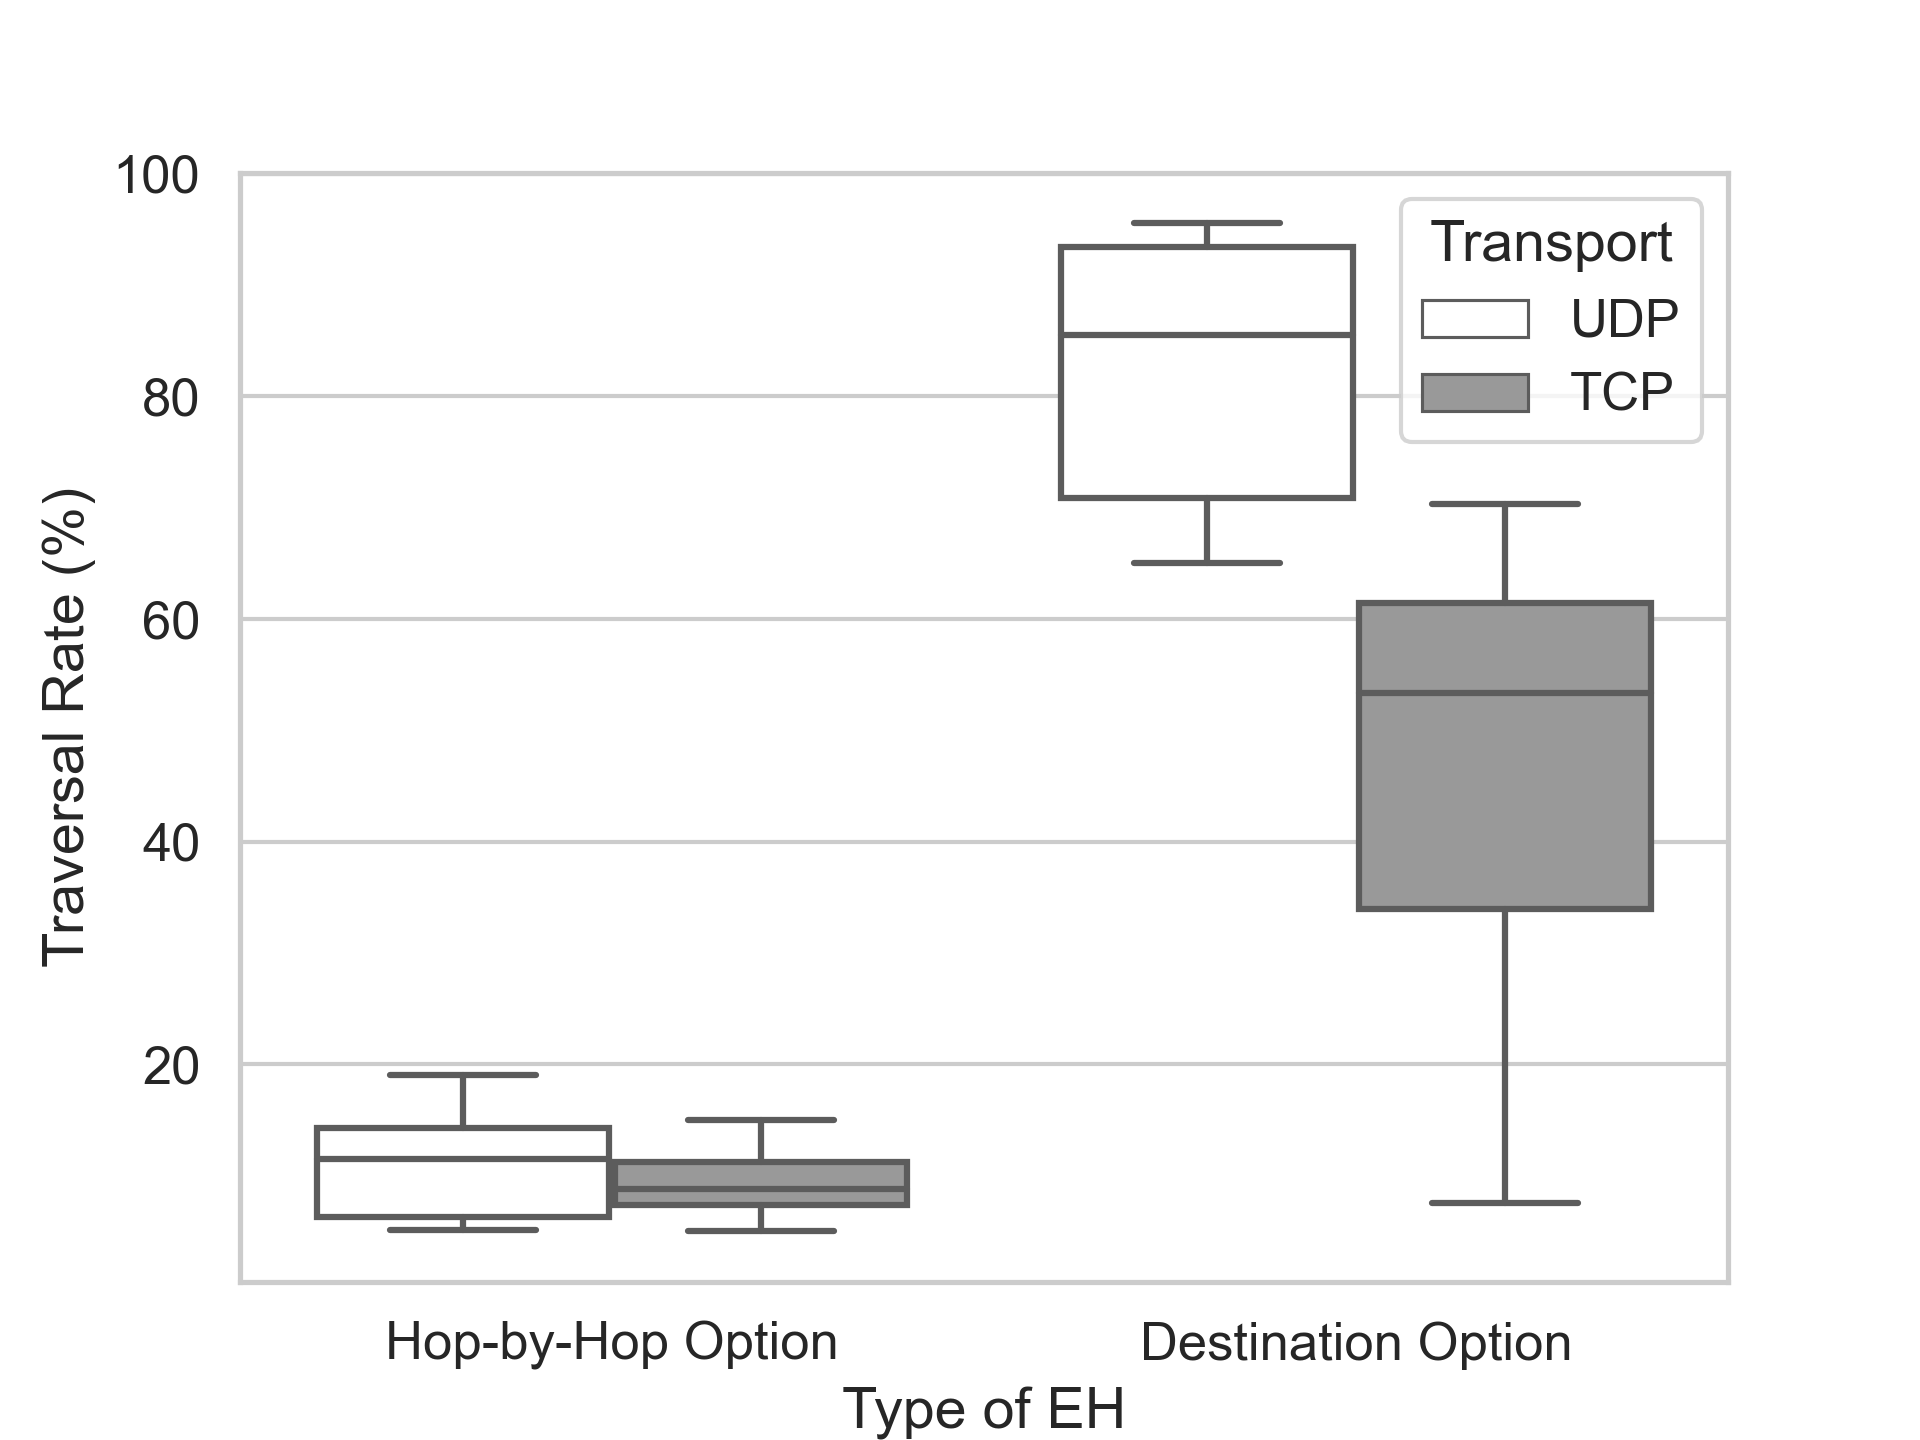
\includegraphics[width=0.5\textwidth]{all_traversal.png}
  \caption{Traversal of HbH and Dest Opts from RIPE Atlas vantage points to target servers located in 7 different countries (dataset R1). }
  \label{fig:countrybox}
\end{figure}

\begin{figure}
\centering
  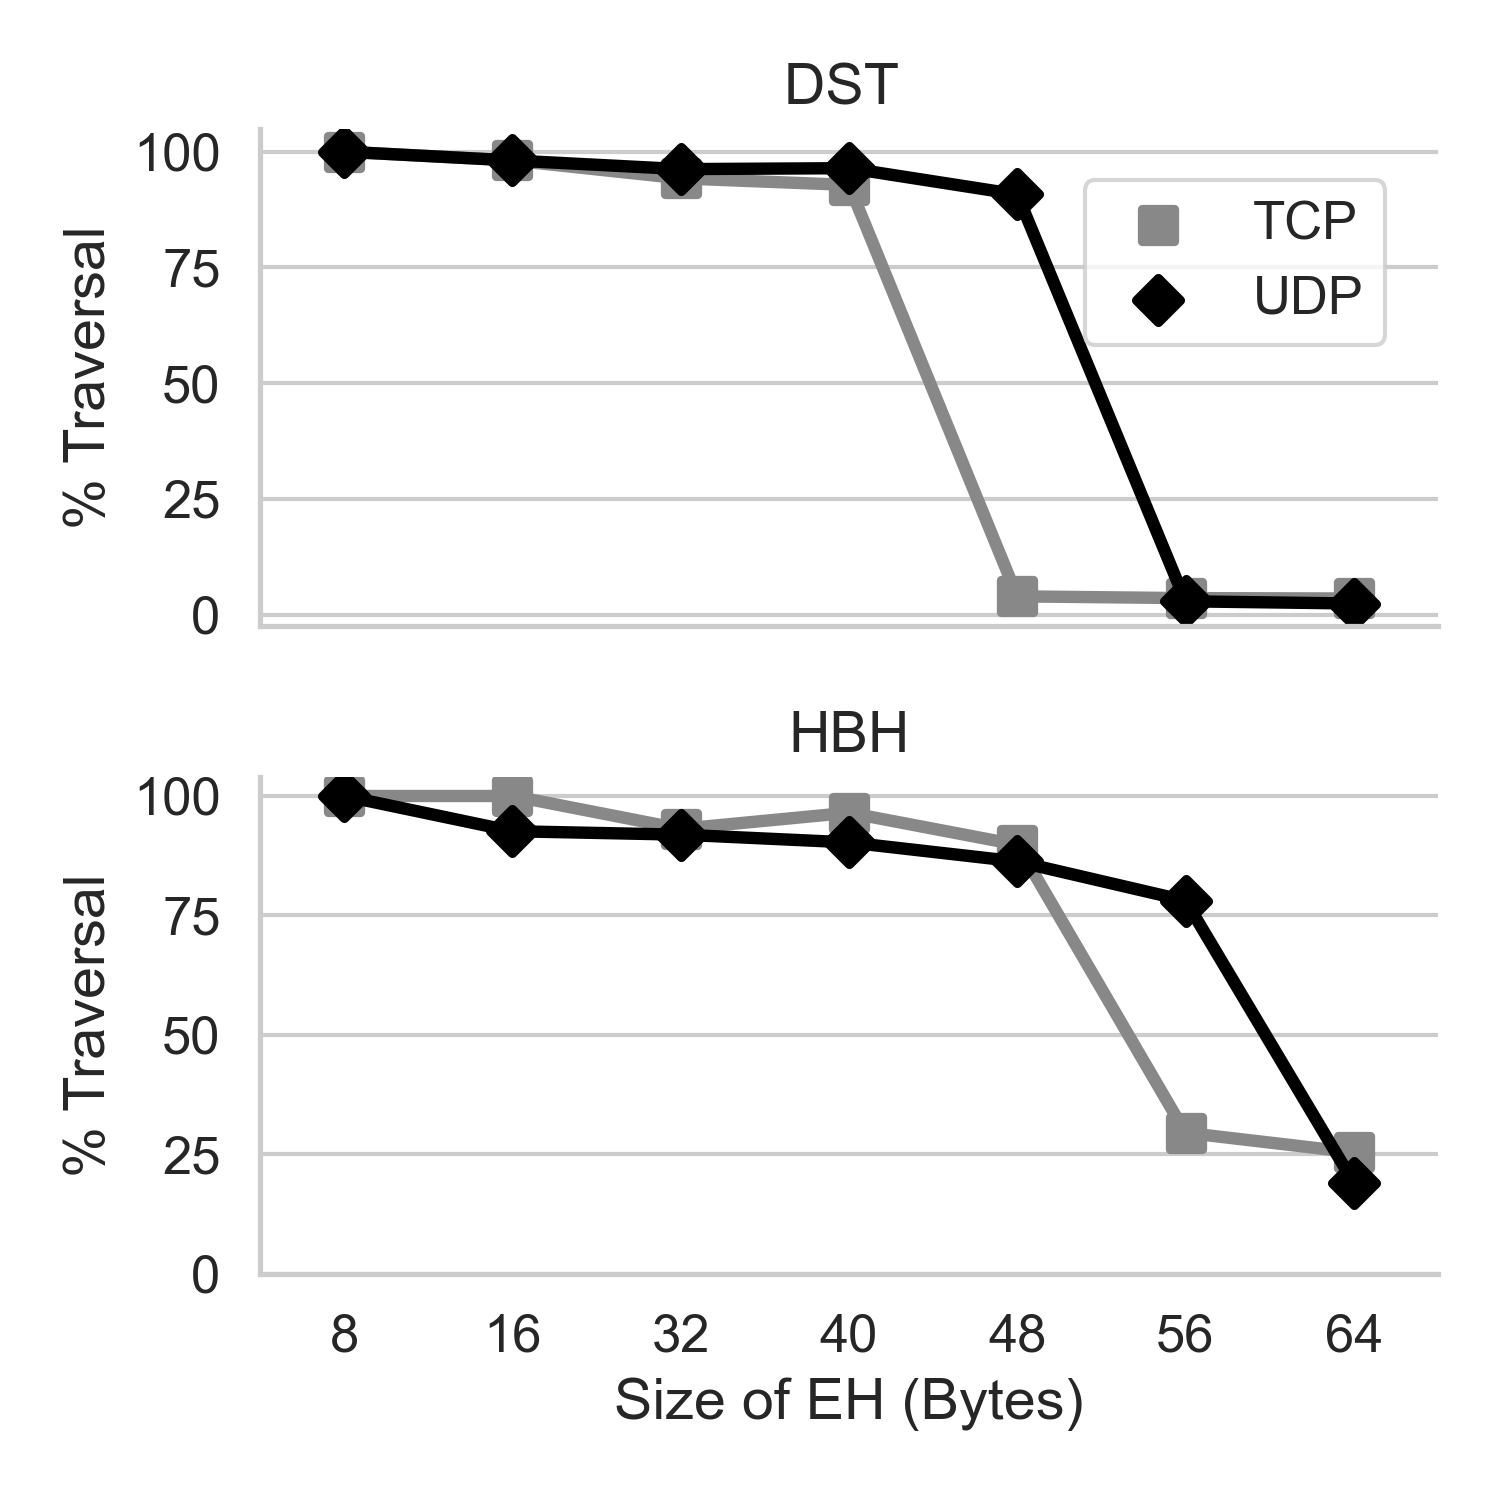
\includegraphics[width=0.45\textwidth]{sizes.png}
  \caption{Traversal percentage of HbH and Dest Opts EHs from RIPE Atlas vantage points to a target server within Janet (AS876), per EH size and split by transport, n=129,585 total measurements, with a mean of 4628 measurements ($\sigma$=351) of for each transport, size and EH combination (dataset R2). The variation in the number of measurements is due to the availability of RIPE Atlas participating probes and changes in probe connectivity over time.}
  \label{fig:sizes}
\end{figure}

\subsection{Pathologies}
    \label{subsec: pathologies}

The results show very low traversal for TCP towards the Kazakhstan and Zambian targets. Both of these target networks have only one BGP peer, and for both, we find that the majority (over 50\%) of TCP packets see their last reply from a router in the destination's upstream AS. In both cases, plotting the path traversal to the AS upstream of the destination AS reveals similar results to targets in other tested countries. This is shown in Figure~\ref{fig:traversal_pathologies}.

\begin{figure}
\centering
  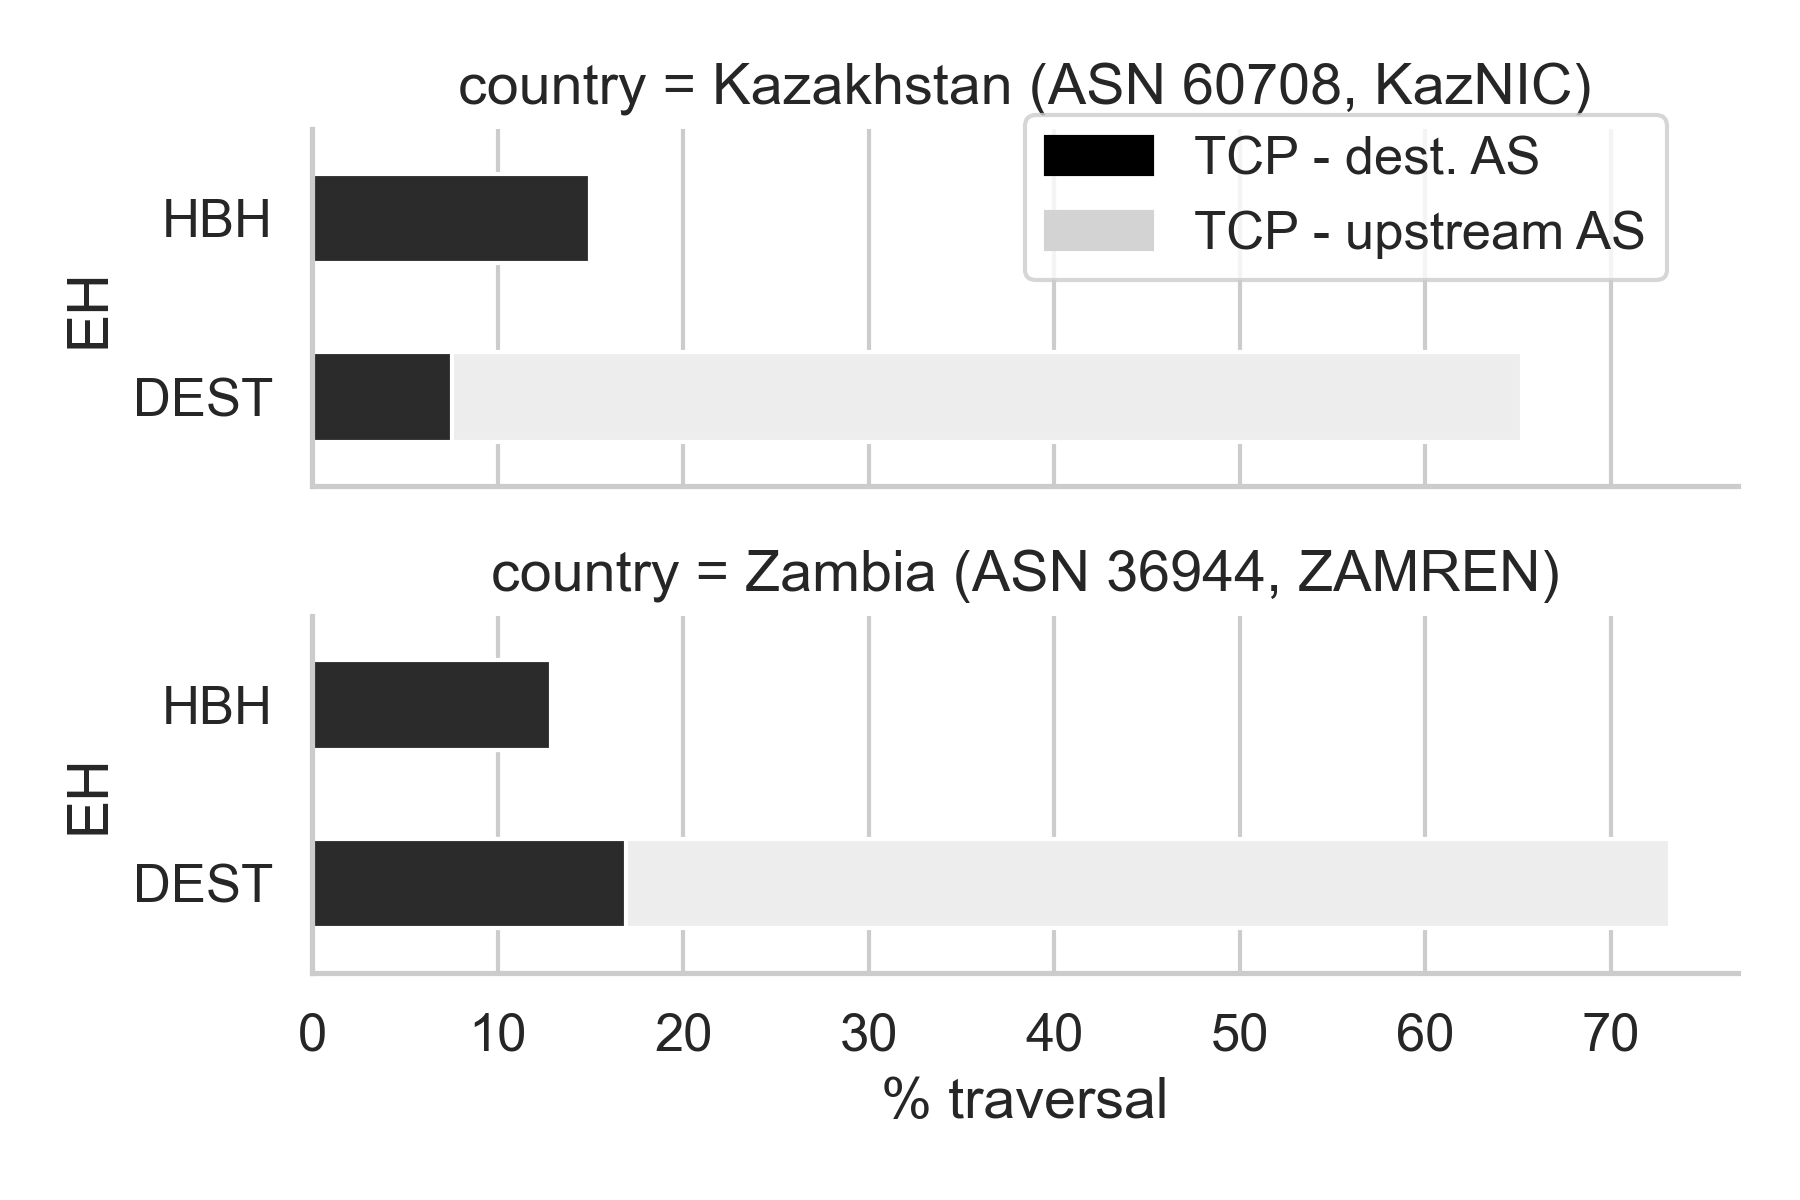
\includegraphics[width=0.5\textwidth]{traversal-pathologies.png}
  \caption{Traversal from RIPE Atlas vantage points to both destination and upstream AS for targets in Kazakhstan (n=5075) and Zambia (n=4462). The figure shows the traversal percentage of TCP packets using both types of tested EH.}
  \label{fig:traversal_pathologies}
\end{figure}

The Kazakhstan network's only BGP peer is Hurricane Electric (AS6939). The baseline measurements reveal the network uses HE's tunnel brokering service - (the IPv6 peering is tunneled over an existing IPv4 connection), using a tunnel endpoint physically located in Dusseldorf. Upon closer inspection, we find that the 7\% of paths where packets traverse to the destination network originate (with 3 exceptions) in ASes located Australia/New Zealand. The 50\% dropped packets that originate in other geographical areas are filtered at the tunnel endpoint. We therefore assume misconfiguration or a policy within the HE transit network routers results in this pathology. 
%They can also come from comcast but somehow they bypass HE?!?!?!?!


The only BGP peer of Zambia's target network is Ubuntunet Alliance For Research and Education Networking (AS36944). Over 50\% of packets are dropped at the last hop seen in this AS. As there is no common origin for the results that do traverse, we attribute the drops to a network filtering device. 

\subsection{Path traversal analysis}

Tables~\ref{tbl:uk_as1} and \ref{tbl:uk_as2} present the traversal percentage of packets with an 8B EH at each AS on the path to the UK destination. We observe the majority of packet drops happen in the first AS on the path (the vantage point AS) - between 68\% HbH Options (UDP) and 74\% (TCP) packets and 5\% (UDP) to 25\% (TCP) of Dest Options packets. The difference due to transport is still prevalent when the results are split per AS. 
We note the source AS drop is common to all RIPE measurements regardless of destination. Dest options over UDP do not see drops greater than 1\% as they further traverse ASes, suggesting they traverse the Internet core.

We further investigate where within the source AS EH packets are discarded, and find the majority of drops happen at the very first router on the path (i.e. the vantage point's local gateway).
Figure~\ref{fig:empty_paths} shows the percentages of paths where packets are dropped at the very first router on the path - i.e. paths where no traceroute responses are received for test packets, but are received for control packets. Packets carrying HbH Options are dropped at the local router on more than 50\% of paths, and this varies very little with transport (54\% for UDP and 56\% for TCP, for an 8B EH). In contrast, only between 2 and 15\% of paths see drops of packets carrying Dest Opts, an this varies with transport (2.5\% for UDP and 10\% TCP for an 8B EH). The drop percentage increases with size regardless of EH used.


The local gateways for this set of vantage points are a diverse mixture of edge routers connecting enterprise LANs, mobile and broadband networks, and which are expected to perform a variety of functions, including access control, authentication or which require transport header information. A common modification made by edge routers is clamping of the Maximum Segment Size (MSS) option in the TCP header. This is done to avoid problems which otherwise arise from Path MTU discovery. 
There is unfortunately no way to determine whether the drops are a result of configuration policy or lack of support. 
However, it is possible to isolate paths that insert TCP options such the MSS option by examining the packets after they arrive at the destination in the baseline measurement. By default, the packets sent with RIPE do not include an MSS option - if present at the destination, this means a device on that path has inserted it.
We identify 853 paths where an on-path device has inserted an MSS option in our baseline measurements to the UK destination. We then look at EH traversal within this subset of paths to determine whether this characteristic makes a difference for the overall traversal percentage, on the basis that at least one on-path device will have needed to parse the entire IPv6 Header, including any EHs, to perform its function.
We find a traversal of only 2.6\% for HbH and 48.1\% for Dest Opts for this subset of paths, indicating dropping is more prevalent where an on-path device that modifies the TCP MSS option exists.


\begin{figure}
\centering
  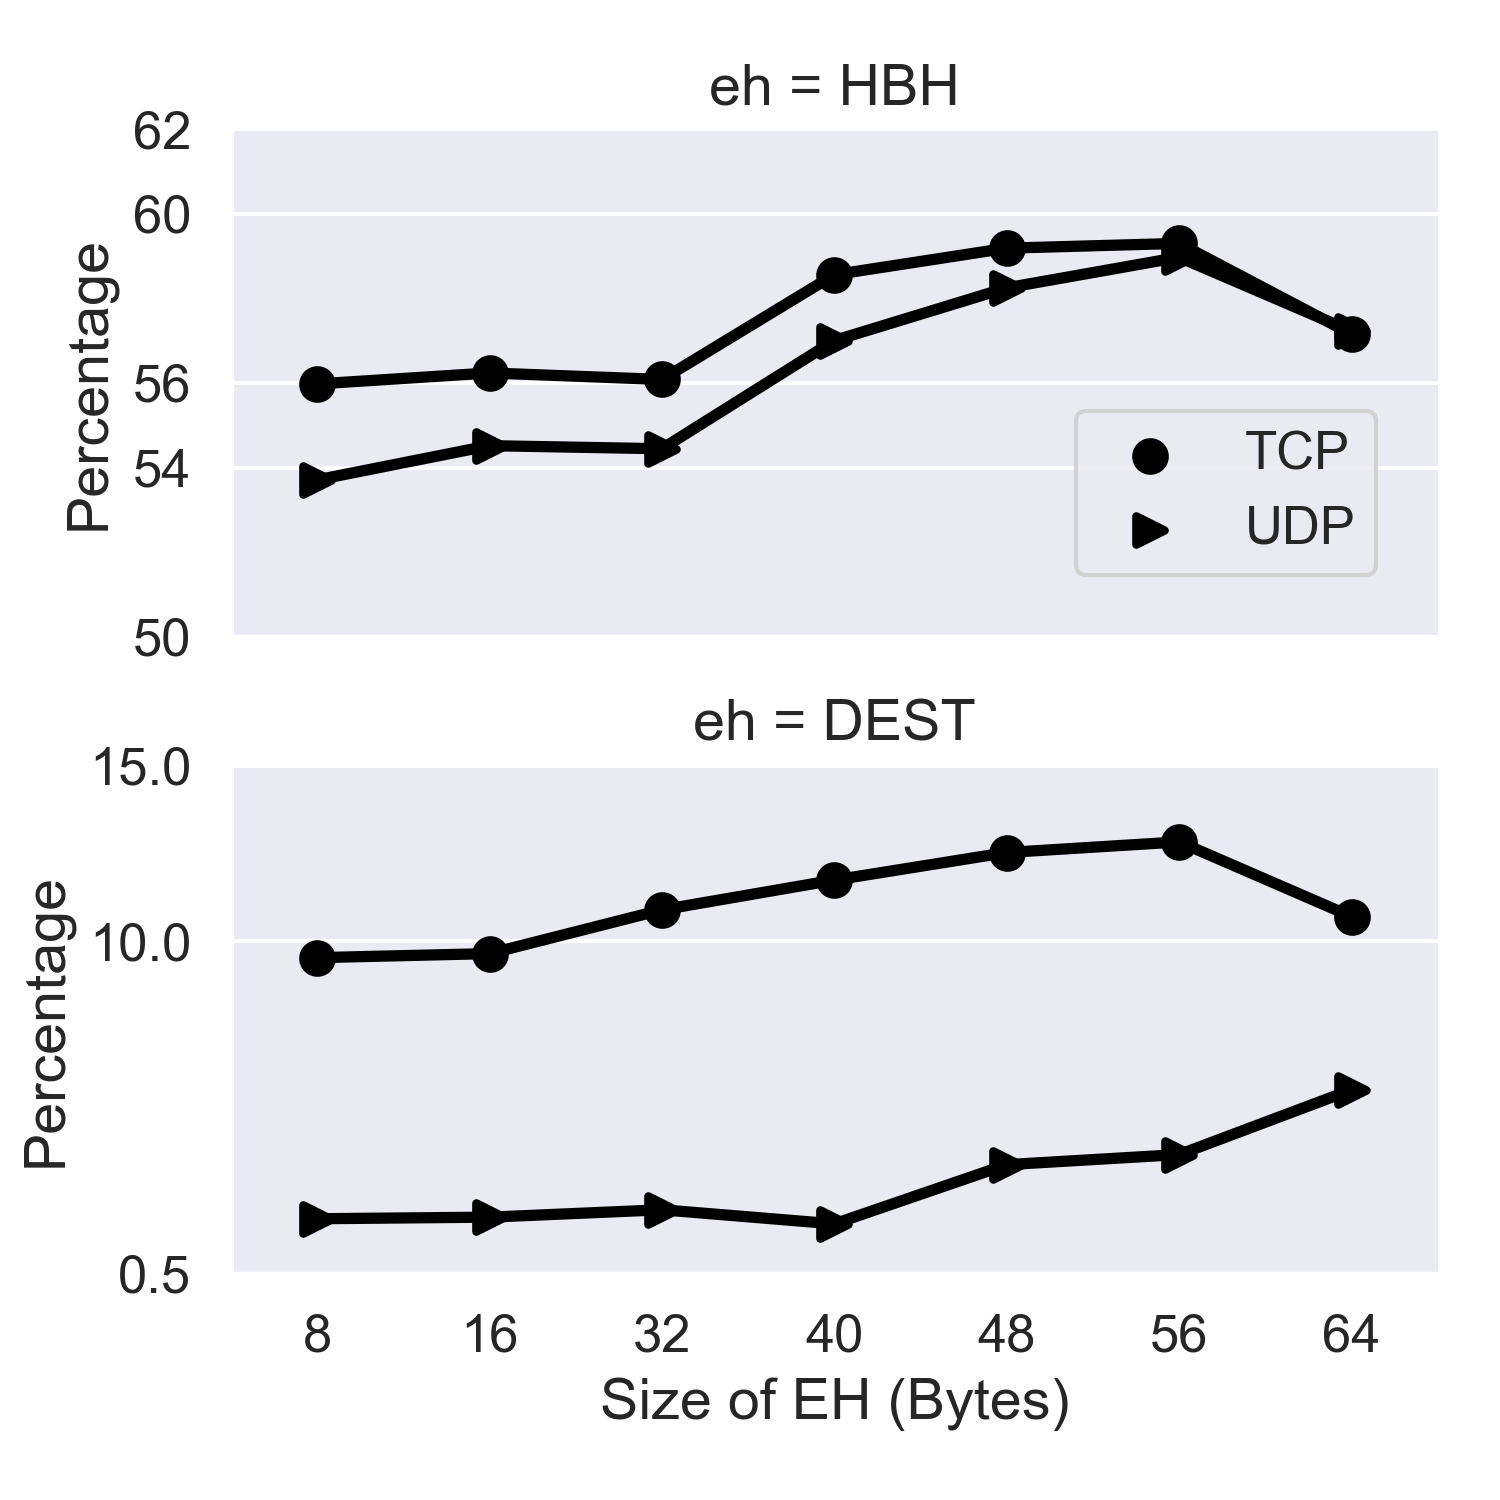
\includegraphics[width=0.5\textwidth]{empty_paths.png}
  \caption{Percentage of paths where packets are dropped at the first router, per EH, transport protocol and size.}
  \label{fig:empty_paths}
\end{figure}


\begin{table}
\centering
\caption{Per-AS drop attribution for 8B Dest Opts packets sent from n=4970 RIPE Atlas vantage points to a target destination in AS786. The local AS is responsible for the majority (5\% for UDP and 25\% for TCP) of the drops.}
 \label{tbl:uk_as1}

\begin{tabular}{l|l|l|l}
                                   & 1st AS & AS1\textgreater AS2 & $inf $     \\ \hline 

{Dest UDP 8B} & 95.3\% & 93\%                 & 91.5\% \\ \hline

{Dest TCP 8B} & 74.7\% & 70\%                 & 68.5\%
\end{tabular}
\bigskip
\caption{Per-AS drop attribution for 8B HbH Opts packets sent from n=4970 RIPE Atlas vantage points to a target destination in AS786. The local AS is responsible for the majority (68\% for UDP and 74\% for TCP) of the drops.}
\begin{tabular}{p{0.07\textwidth}|l|l|l|l|l}

              & 1st AS & AS1\textgreater{}AS2 & 2nd AS & AS2\textgreater{}AS3 & $inf$     \\ \hline
HbH UDP 8B & 31.4\% & 20.1\%               & 15\%   & 12.2\%               & 11.4\% \\ \hline
HbH TCP 8B & 26.9\% & 16.3\%               & 13.9\% & 9.7\%                & 8.6\%  \\ 
\end{tabular}
 \label{tbl:uk_as2}
\end{table}


\subsection{Internet path analysis}

Load balancing routers are another type of on-path devices that can operate on the upper layer headers of a packet. To determine whether this function is impacted by packets with EHs, we perform Paris Traceroute measurements. This tool aims to detect the presence of load balancing on a given path~\cite{augustin2006avoiding}, by performing multiple traceroute measurements varying several header fields (a `Paris variation'); on-path devices may use several of these fields for load-balancing purposes. To identify the packets sent for a specific measurement, Paris Traceroute relies on  TCP's sequence number field or the checksum field in the case of UDP.

We run 6 sets of measurements from RIPE Atlas vantage points to the Zambian destination, with each set using 16 Paris variations. We carefully select the vantage points and destination based on previous measurements, so as to only measure complete paths, where traversal always succeeds. We find a total of 866 paths. The Paris Traceroute version used by RIPE Atlas varies the IPv6 Flow Label and transport port number deterministically between individual Paris measurements. Each group of 16 Paris measurements is considered a measurement set. The same 16 combinations of IPv6 Flow Label and port number are used for subsequent measurement sets.

\begin{figure}
\centering
  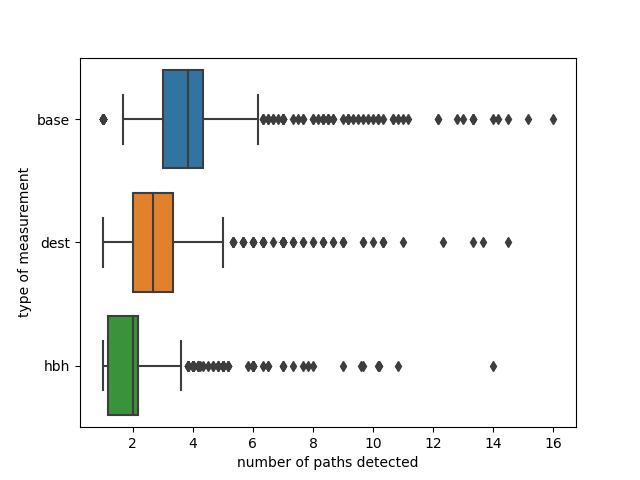
\includegraphics[width=0.5\textwidth]{boxplot-paths-detected.png}
  \caption{Number of paths detected by Paris Traceroute in 866 source-destination pairs, averaged over 5 measurement runs, with each run using the same 16 Paris variations. The baseline measurement using vanilla packets is compared against Dest and HbH Opts measurements (dataset R3).}
  \label{fig:paths-detected}
\end{figure}

Figure~\ref{fig:paths-detected} compares how many paths are discovered by Paris Traceroute when using vanilla IPv6 packets versus packets that contain an 8B Dest or HbH Opts EH.
A total 16 Paris variations discover on average 4 paths~\cite{augustin2006avoiding}. We reproduce this in our baseline results, finding a median of 4.1 paths. However, the medians for measurements where packets carried an 8B Dest or HbH Opts EH are 2.96 and 2.1 respectively (Figure~\ref{fig:paths-detected}).

For 518 (60\%) of source-destination pairs, measurements performed with Dest Opts EHs detect the same (+-1 path) number of paths as the baseline. For 328 (38\%) pairs, the measurements detect fewer (by 1 path or more) number of paths than the baseline. On the other hand, measurements using HbH Opts EHs detect the same (+-1 path) number of paths as the baseline for only 115 (13.4\%) source-destination pairs. Much more commonly, fewer paths are detected when this type of EH is used compared to the baseline. This happens on 604 paths (69.7\%). This pathology could happen, for example, if ECMP-enabled routers use a byte offset for their hash calculations. Overall, this means that packets with an HbH EH are less likely to take the same internet path as a vanilla packet.

For some source-destination pairs, the EH Paris measurements detect at least 1 more path than the vanilla measurements. These cases are rare - around 1\% (8 paths for Dest Opts and 10 for HbH Opts), but can however reveal interesting pathologies.
For example, for one pair the baseline measurement detects 4 paths, the Dest Opts measurement detects 2 paths, while the HbH measurement detects 14(!) different paths. Upon closer inspection we find a single router that enumerates 14 interfaces, only in the presence of packets containing HbH EHs.
%For 12 source-destination pairs in the dataset, not enough data was gathered using Destination Option EHs to complete a measurement run. Not enough data was gathered for 137 (15.8\%) pairs.
This set of measurements indicates that not all load balancer implementations are well suited for packets carrying the HbH or Dest Opts EH.


\section{Pathspider results} 
\label{sec:pathspider-results}

This section presents results obtained with PATHspider. In contrast to the RIPE Atlas tests, these experiments use a limited number of vantage points and target a large number of destinations. Where the destination is an authoritative NS, PATHSpider first performs a control measurement by sending a DNS query to the server using vanilla IPv6 packets. The same measurement is then repeated using an 8 Byte PadN Dest or HbH Opts, and in each case the test is considered successful if the server replies to the DNS query. Where the destination is a web server, the test can only be done over TCP by sending a TCP SYN, and is considered successful if the server replies with a TCP SYN-ACK.
This section reports on the end-to-end support, or the percentage of paths where test packets were observed to receive a response from the destination server.

\begin{table} 
\begin{tabular}{c|cc|cc}
\multicolumn{1}{l|}{} & \multicolumn{2}{c|}{Dest Opts Support} & \multicolumn{2}{c}{HbH Opts Support} \\ \cline{2-5} 
\multicolumn{1}{l|}{} & \multicolumn{1}{c|}{TCP}       & UDP      & \multicolumn{1}{c|}{TCP}     & UDP     \\ \hline
UK                    & \multicolumn{1}{c|}{69.1}      & 69.3    & \multicolumn{1}{c|}{12.5}    & 15.8  \\ \hline
Canada                & \multicolumn{1}{c|}{76.3}      & 76     & \multicolumn{1}{c|}{23.3}    & 24.2  \\ \hline
Australia             & \multicolumn{1}{c|}{72.5}        & 72.2      & \multicolumn{1}{c|}{17.7}    & 17.5  \\ \hline
Singapore             & \multicolumn{1}{c|}{72.8}      & 72.7    & \multicolumn{1}{c|}{17.4}    & 17.4   \\ \hline
Poland                & \multicolumn{1}{c|}{76.5}      & 76.8   & \multicolumn{1}{c|}{24.4}    & 24.7   
\end{tabular}
\label{tbl:e2e_traversal}
\caption{End-to-end support for an 8B Pad N option for both Dest and HbH EHs, from vantage points in 5 countries to n=18002 unique authoritative NSes in the Cisco Umbrella Top 1M, in 2787 different known ASes. All measurements performed in February 2023, part of dataset P1. }
\end{table}

\begin{table} 
\begin{tabular}{c|c|c|c}
           & \% of dataset & Supports Dest Opts & Supports HbH Opts \\
\hline
Cloudflare & 18                      & Yes                & No                 \\
\hline
Amazon     & 11                     & No                 & No                 \\
\hline
Hetzner    & 3                     & Yes                & No                 \\
\hline
Gandi      & 4                     & No                 & No                 \\
\hline
Ionos      & 3                    & Yes                & No                
\end{tabular}
\label{tbl:provider_support}
\caption{End-server support for the Dest and HbH Opts for major DNS server providers, n=99,987 paths, based on measurements from December 2022. Google does not support either option, and is not listed in the table as it only had 30 destinations in the dataset.
}
\end{table}

\subsection{End-to-end support}
\label{subsec:e2esupport}

Table~\ref{tbl:e2e_traversal} presents the end-to-end support for the authoritative NSes for the current Cisco Umbrella top 1M Domains list (Feb 2023).
% ANA TODO - double check results^

As with the access network results previously presented, support varies between the Dest and HbH EHs: 69 to 80\% of the tested servers replied to packets using Dest Opts, and up to 24.2\% do so for HbH Opts. Traversal does not vary with transport in the same way seen for the access network results presented in the previous section. We attribute this to the lack of edge router devices normally present in access networks. Only one measurement, from the Singapore vantage point, sees a 5\% difference based on transport in favour of TCP for both EHs tested.
Finally, the table shows variations in support based on vantage point - support varies between 12 to 24.7\% for HbH Opts, indicating fewer packets dropped in transit networks in the latter case.

However, around one third of destinations in the DNS dataset featured in Table~\ref{tbl:e2e_traversal} are hosted by a few major hosting companies (Cloudflare, Amazon, Gandi etc.) which employ network policies to filter packets with some EHs in their network. End-server support for major DNS server providers are presented in Table~\ref{tbl:provider_support}. In Early December 2022, Cloudflare servers started responding to DNS queries send over packets with Dest options, resulting in a jump from 57\% to over 70\% for the dataset. If all major providers would enable support, this would bring the success of the E2E test to over 90\% for Dest Opts and 60\% for Hbh Opts for this dataset.

We tested end-to-end support for webservers in the Cisco Umbrella top 1M Domains list (232350 unique IP addresses, Feb 2023) from the same destinations. This list of webservers is much more dominated by a few major hosting companies: around 52\% of destinations are hosted by Amazon Inc (AS16509); 23\% are hosted by Cloudflare (AS13335), and around 2.5\% each are hosted by Akamai Technologies and Google. We break down supported EHs for each in Table~\ref{tbl:web_provider_support}. We find more than two-thrids of Amazon-hosted webservers respond to connections over packets with Dest Opts, in contrast to Amazon-hosted DNS servers, where none do. 

Overall, we find end-to-end support for all tested webserver addresses to be between 72 and 78\% for Dest Opts packets and between 2-3\% for HbH Opts.


\begin{table} 
\begin{tabular}{c|c|c|c}
           & \% of dataset & Supports Dest Opts & Supports HbH Opts \\
\hline
Amazon & 52                      & Yes                & No                 \\
\hline
Cloudflare     & 23                     & Yes                 & No                 \\
\hline
Akamai    & 2.7                     & Yes                & No                 \\
\hline
Google      & 2.3                     & No                 & No                 \\
\
\end{tabular}
\label{tbl:web_provider_support}
\caption{End-server support for the Dest and HbH Opts for major webserver providers, n=99,987 paths, based on measurements from December 2022. Google does not support either option, and is not listed in the table as it only had 30 destinations in the dataset.
}
\end{table}


\subsubsection{Option Type support}

We repeated the DNS server experiment described above from one vantage point, varying the Option Type and Option Lnegth fields. 
Table~\ref{tbl:option_type_support} shows the support for different Option Types within the authoritative NSes for the current Cisco Top 1 Million Domains. We test a well-known option, PadN~\cite{rfc2460}, against a recently-standardized one - Minimum Path MTU HbH Option~\cite{rfc9268}. We also test two experimental options, 30 and 254~\cite{RFC4727}. The latter was chosen to test the traversal behaviour where the Option Type has its two most significant bits set.
We find that the Option Type does not affect traversal where the two most significant bits of the field are not set - with the same traversal percentage for PadN, PMTU Discovery and Experimental Option 30. Where the highest order bits are set, traversal is expected to be 0 - however, we still receive responses on 0.4\% of paths, indicating all devices on that path have ignored these bits.

The same applies for an incorrectly set Option Length field. As any device parsing the EH field should validate the Option Length set for each option, traversal is expected to be 0; however we still find a small number of paths (0.5\%, or around 80 paths) where all devices on the path ignore this field.

\begin{table}
\begin{tabular}{l|l|l}
Test                      & Dest Options EH & HbH Options EH \\
\hline
Pad N option (1)          & 69.3           & 15.1          \\
PMTU Discovery (48)       & 69.5           & 15.8          \\
Experimental Option (254) & 0.4            & 0             \\
Experimental Option (30)  & 69.4           & 15.1          \\
Incorrect Option Length   & 0.5            & 0.05            
\end{tabular}
\label{tbl:option_type_support}
\caption{End-to-end support for different Option Types in the authoritative NSes for the Cisco Top 1 Million Domains, n=19052 unique IPv6 targets. The transport used was UDP (dataset P2).}
\end{table}

\subsubsection{ICMP Unreachable Messages}

When a packet with a HbH Opt is sent but does not receive a reply (i.e. the packet is dropped on path),  ICMP unreachable messages are seen on 0.2\% of the tested NS paths. For Dest Opts packets, ICMP unreachable messages are seen on between 0.3 and 8.8\% of paths, depending on vantage point.
This suggests that ICMP messages cannot be used to ascertain whether a packet carrying options was dropped in transit.
Upon closer inspection, we also find that for all destinations, ICMP unreachable messages can be received even when the test succeeds on up to 2\% of paths. These are exclusively received from routers in destination ASes and indicate misconfiguration.


\subsubsection{ICMP Parameter Problem Messages}

When a packet carries a Dest or Hbh Option which has its two MSBs set, routers that do not understand this option should discard packets with this option and return an ICMP Type 4 Parameter Problem message back to the sender. To examine whether this is prevalent in the Internet, we repeat the DNS server experiments using packets using experimental Option Type 254. This option has its two MSBs set and is unlikely to be understood by any routers, and therefore we expect any sent packets to be dropped.

Behaviours for Dest Opts and HBH Opts respectively are described in Table~\ref{tbl:icmp_support_dst}.

In the case of Dest Options, for all vantage points tested, only the gateway router local to the vantage point returns ICMP Type 4 Parameter Problem messages for the packets sent, as expected; the percentage of destinations for which the ICMP messages are received varies between 50-100\%. As the local router always generates these messages, we attribute this variation to ICMP rate limiting. 

In the case of Hop-by-hop options, we find that while the local gateways in all vantage points forward the packets,  ICMP Type 4 Parameter Problem messages are received from intermediary routers on the path or in the destination AS. The response rate varies between 52 and 73\%. 

For both EHs tested, due to ICMP rate-limiting and filtering, this mechanism is not found to be a reliable indicator on whether or not a packet with an unknown option with its two MSBs set is dropped. We also find that on many paths, packets with Hop-by-Hop Options are forwarded nevertheless.

In addition, for Dest Opts packets, on between 0.2 and 0.5\% of paths, we also find that despite sending this message, the local router also forwards the packets to the destination and a response is still obtained by the server (the end-to-end test succeeds), which could indicate a router implementation issue.

\begin{table}
\begin{tabular}{p{0.12\textwidth}|p{0.04\textwidth}|p{0.03\textwidth}|p{0.03\textwidth}|p{0.03\textwidth}|p{0.03\textwidth}|p{0.025\textwidth}}

\centering

                                           &             & UK        & Can       & Aus    & Sgp          & Pol     \\
                                           \hline

{\% ICMP received in vantage AS}        & {HBH DEST} & {0 100}  & {0 51.6}    & {0 51.9}    & {0 51.9}    & {0 51.5}  \\
\hline
{\% ICMP received elsewhere on path}          & {HBH DEST} & {72.8 0} & {52.5 0}    & {68.2 0}    & {69.2 0}    & {73  0}    \\
\hline

{\% ICMP received, packet forwarded}          & {HBH DEST} & {0 0.52} & {0 0.48}    & {0 0.46}    & {0 0.24}    & {0 0.46}  \\
\hline

{\% ICMP message not received} & {HBH DEST} & {27.2 0} & {47.5 48.4} & {31.8 48.1} & {30.8 48.1} & {27 48.5} 
\end{tabular}
\caption{Different behaviours for ICMP rate-limiting.}
\label{tbl:icmp_support_dst}
\end{table}

\subsubsection{Longitudinal support}

Table~\ref{tbl:longitudinal_support} presents measurements over the same set of domains over the course of 3 years. The domains were resolved prior to each measurement, resulting in a variation of the total unique IP addresses tested, presented in the last table row. The results show a trend towards lower support for HbH Opts, with Dest Opts support remaining constant over time, until December 2022 when Cloudflare enables support as described in Subsection~\ref{subsec:e2esupport}.

% Ana: verify total number of paths.
\begin{table}
\begin{tabular}{l|l|l|l|l}
                    & Jan 2020 & Jul 2020 & July 2022 & Dec 2022 \\
\hline
Dest Opts & 59.9\%   & 54.3\%   & 57.4\%    & 71.7\%   \\
HbH Opts  & 25.7\%   & 23.8\%   & 16.4\%    & 11.9\%   \\
\hline
Unique IP addresses & 18296    & 19690    & 19553     & 20050   
\end{tabular}
\label{tbl:longitudinal_support}
\caption{End-to-end support for an 8B Pad N option for both Dest and HbH EHs, from one vantage point to the authoritative NSes for the same set of 1M domains, between Jan 2020 and Dec 2022 (dataset P1). The transport used was UDP.}
\end{table}

\subsection{AS analysis }

Pevious figures show end-to-end server support. We note that end-to-end support is not the same metric as path traversal. The latter is concerned with whether packets reach the destination AS.

Table~\ref{tbl:as_pathspider} presents ASes targeted by Pathspider (2868 in total) alongside evidence that they support either the Dest or HbH EH.
If at least one reply is seen from that AS to one of our test packets from any of the locations tested, we consider that AS supports the traversal of packets using the tested EH type. Thus, at least 92.4\% of destination ASes allow traversal of packets carrying an 8B Dest Opts EH, and more than half, 53.8\%, allow an 8B HbH Options EH. The percentage drops when we consider multiple paths towards that AS, revealing that many packets carrying EHs are dropped in en-route in an AS different from the destination AS. For Dest Opts, 3.4\% fewer ASes support Dest Opts on more than half the paths, whereas for HbH Opts, the difference is 16.6\%.
When only considering the subset of ASes (1606) tested over 10 or more paths, the results vary little: at least 93.2\% of destination ASes allow traversal of packets carrying an 8B Dest Opts EH, and more than half, 55.9\%, allow an 8B HbH Opts EH.

    \begin{table}
\begin{tabular}{p{0.195\textwidth}|p{0.11\textwidth}p{0.118\textwidth}}
                                          & Paths per AS$>$=1 & Paths per AS$>$=10 \\ \cline{1-3} 
Total number of ASes                      & 2787                                            & 1606                                            \\ \hline
AS does not support Dest Opts               & 212 (7.6\%)                                     & 110 (6.8\%)                                     \\
AS supports Dest Opts on 1 or more paths   & 2575 (92.4\%)                                   & 1496 (93.2\%)                                   \\
AS supports Dest Opts on 50\% paths or more & 2476  (88.8\%)                                  & 1437 (89.4\%)                                   \\ \hline
AS does not support HbH Opts               & 1287 (46.2\%)                                   & 709 (44.1\%)                                    \\
AS supports HbH Opts on more than 1 path   & 1500 (53.8\%)                                   & 897 (55.9\%)                                    \\
AS supports HbH Opts on 50\% paths or more & 1037 (37.2\%)                                   & 580 (36.1\%)                                   
\end{tabular}
\label{tbl:as_pathspider}
\caption{Number of ASes where DNS servers can be reached via packets carrying either Dest or HbH Opts. The first column considers all destination ASes in the dataset, while the second only looks at ASes that host 10 destinations or more. Based on measurements from December 2022 (dataset P1).}
\end{table}

\section{Discussion} 
\label{sec:discussion}

Since its standardisation, the IPv6 protocol has
seen widespread adoption~\cite{v6adoption_ton} and the hardware and software to
support it have matured: packet lookup capacity in routers is increasing and
router architectures have evolved, with solutions based on re-configurable
logic circuits that allow specific and dedicated functions now
emerging~\cite{cisco-silicon-one}.

Updates have also been made to the IPv6 standard itself based on this
operational experience~\cite{RFC5722}~\cite{RFC6734}~\cite{RFC6564}~\cite{RFC8200}. These improvements continue as EH processing has become a recent focus in the standards community, aiming to motivate a change in both network operator policies and the implementation of more resilient router architectures that facilitate EH processing~\cite{ietf-6man-hbh-processing-06, ietf-v6ops-hbh-03, ietf-6man-eh-limits-02}. 


%Question 1: do extension header actually traverse common Internet paths? Is there a longitudinal trend making this more easy or harder?
We find that packets with EHs traverse Internet paths in many cases, and that many ASes allow support.
Packets with HbH Opts are still dropped in many transit networks (as validated on paths to server edge networks in Table~\ref{tbl:as_pathspider}) and in access networks in Figure~\ref{fig:countrybox}. Misconfiguration or other network policies can result in pathologies within transit networks as shown in Subsection~\ref{subsec: pathologies}. We also find that traversal drops significantly on paths containing edge-network devices which insert a TCP transport option.

Server-side, testing the same set NSes between 2019 and 2022 reveals the support for 8B PadN HbH Opts decreases over time when considering individual destinations (Table~\ref{tbl:longitudinal_support}) as more NS servers become centralised under only a few ASes that do not support HbH Opts.  However, an AS analysis reveals more than half of the tested ASes allow packets carrying a HbH Opts EH and more than 90\% allow packets carrying a Dest Opts EH. The AS analysis confirms that transit networks can represent a barrier to deployment for the HbH Opts EH.
 
RFC 7872~\cite{RFC7872} describes the traversal to the authoritative NSes for the Alexa Top 1M domains in 2014. They find packets carrying an 8B PadN Dest Opt traverse to 78.6\% of destinations and packets carrying an 8B PadN HbH Opts traverse to 45.9\% of destinations. Their results are obtained from a single vantage point and are not grouped per AS and so can be compared with results in Table~\ref{tbl:longitudinal_support}.
This indicates an a small decrease in support for Dest Opts and a larger decrease in support for HBH Opts on paths to NS servers, although this may reflect changes within the top 1M domain list itself between 2014 and 2023.
Also, our AS analysis reveals that packets with Options traverse to up to 90\% and over 50\% of ASes respectively, and so we can infer the decrease is due to drops within the destination AS.

%Question 2: is there a limit to extension headers that prevents them from traversing certain Internet paths such as limiting length of the EH chain or a specific EH length? Would ? Is it different between HBH and DO?

EHs up to 40B in size sent over UDP have the highest chance of traversing access network paths, as shown in Figure~\ref{fig:sizes}, for a total IPv6 header and transport chain of under 104B. This suggests that when using EHs, keeping packet sizes under this limit may help in ensuring consistent deployment.

%Question 4: is there a possibility to deploy a different new option...is this sensitive to the format of the option or the presence of a new defined option? This is a part whether a specific option causes the traverse ability to change, or whether an illegal format option changes the traversability of the packet.

We also find that traversal does not depend on the type of option sent (see Table~\ref{tbl:option_type_support}) and so any new specified Dest or HbH Opts (such as the Min. PMTU Discovery Option~\cite{rfc9268}) will not be automatically dropped and their traversal will not depend on changes to deployed infrastructure.

%Question 3: When options extension headers do traverse, do they traverse consistently for the same pair of endpoints? Is %the flow label a help in ensuring a consistent set of network devices on a path?
%Is there a trend to set meaningful entropy in the flow label against the original place where many endpoints sent a zero value flow label?
%Here we should not forget the proposals to add flow metadata as a hop by hop extension to let network devices know helpful information to consider how to fold the packets in a flow.

%Question 5: If we find HBH options don’t work everywhere then ….What is the opportunity for using a hop by hop extension header on some of the packets belonging to a flow? does this result in new forwarding pathologies? That is where the packets with extension headers take a different set of devices to the packets without extension headers, and if so do they take a different network or do they simply follow a different path through the same operator network? Does this result in inconsistent loss? Is the option useful ?

Results presented in Figure~\ref{fig:paths-detected} show that adding an option to a packet may change its forwading path. We note that both the Flow Label and the source port of packets were varied to detect paths between the same pair of endpoints. EHs sit between the IPv6 header (which contains the flow label) and the transport header (which contains the source port), suggesting some load-balancing networking equipment use a byte offset which is expected to contain the source port, and that the flow label is not used in all cases. Overall, this means traffic flows that mix packets with these EHs and packets without must take care as these may not travel on the same Internet path.


%Question 6: what is the opportunity for destination options? Is it a good trade-off to have a network layer? That is consistent transport header or is it wiser to put the transport header information within the transport and therefore allow it to be encrypted such as quic transport parameter - so what is the real advantage of destination options?

---




%Our results also show that most routers are configured to discard packets and send ICMP messages as specified by~\cite{RFC4443} when encountering an option that cannot be processed.However, we still find instances where a router sends this message in response to a Dest Opts EH that has both most significant bits set, but packets are forwarded nevertheless; a more common pathology is forwarding HbH Opts EH packets with both most significant bits set without sending an ICMP message.


\section{Conclusion}
\label{sec:conclusion}

We  find traversal of HbH and Dest Opts is variable depending on EH, size, transport and type of network. We find these EHs can impact the function of load balancing routers and devices that modify the TCP MSS options and that deploying them in the Internet needs to take into account the type of network these will operate over.


\bibliographystyle{abbrv}
\small
\bibliography{main,rfc}


\end{document}
